\section{\textcolor{red}{ Problemas no controle corporal}}

%%%%%%%%%%%%%%%%%%%%%%%%%%%%%%%%%%%%%%%%%%%%%%%%%%%%%%%%%%%%%%%%%%%%%%%%%%%%%%%%
%%%%%%%%%%%%%%%%%%%%%%%%%%%%%%%%%%%%%%%%%%%%%%%%%%%%%%%%%%%%%%%%%%%%%%%%%%%%%%%%
%%%%%%%%%%%%%%%%%%%%%%%%%%%%%%%%%%%%%%%%%%%%%%%%%%%%%%%%%%%%%%%%%%%%%%%%%%%%%%%%
\subsection{\textcolor{red}{Dançar saltitando}}
\index{Problemas!Saltitar}

\begin{problemT}[Saltitar quando dançamos:]
Eu percebo que o saltitado na dança de uma pessoa pode ter em alguns casos um origem mental e em outros um origem físico.
\begin{itemize}
\item \textbf{Mental:} Algumas vesses, o saltitar na dança de uma pessoa, 
é o jeito que esta tem para conseguir  seguir o pulso e ritmo de uma música. 
Isto, quando a pessoa ainda não entende conscientemente estes conceitos.
\item \textbf{Físico:} Outras vesses o saltitar na dança é produto que a pessoa se movimenta na dança,
com o peso do corpo dividido em ambos pés, de modo que quando esta deseja movimentar algum pé,
a pessoa tem muita dificuldade de tirar este pé do chão; 
pois sem importar que pé escolha na movimentação, a pessoa perderá o equilíbrio,
pelo que para movimenta-se na dança esta desenvolve o saltitar; é dizer, 
fazer efeito mola nos joelhos ao igual que os dançarinos de ``swing'', 
para que no momento que estiquem os joelhos a pessoa tenha uma oportunidade de movimentar algum pé.    
\end{itemize}
\end{problemT}


\begin{SolutionT}[Relativa ao problema de saltitar:]
Para solucionar o saltitar na nossa dança devemos nos perguntar se o origem é mental, físico ou ambos;
neste sentido devemos ter em conta as seguintes recomendações:
\begin{itemize}
\item  Aprender a reconhecer o tempos fortes e o pulso, 
libera à pessoa da necessidade de levar o ritmo usando saltos.
Porem, mesmo depois de entender conceitualmente e identificar perfeitamente o pulso musical,
é possível que a pessoa ainda tenha o vicio de saltitar, mesmo que já não seja necessário;
neste caso a solução é identificar este vicio e segurar ele em danças, 
onde nosso único foco de treinamento seja não realizar estes saltos, ate perder essa costume.
\item  Treinamentos atribuindo o peso do corpo completamente a um pé, 
enquanto nos movimentamos, primeiro sem acompanhamento musical,
e logo seguindo a música, 
nos ajudará a ganhar a costume de ter o peso do corpo definido num pé,
antes de animar-nos a movimentar u outro. 
\end{itemize}
\end{SolutionT}




%%%%%%%%%%%%%%%%%%%%%%%%%%%%%%%%%%%%%%%%%%%%%%%%%%%%%%%%%%%%%%%%%%%%%%%%%%%%%%%%
%%%%%%%%%%%%%%%%%%%%%%%%%%%%%%%%%%%%%%%%%%%%%%%%%%%%%%%%%%%%%%%%%%%%%%%%%%%%%%%%
%%%%%%%%%%%%%%%%%%%%%%%%%%%%%%%%%%%%%%%%%%%%%%%%%%%%%%%%%%%%%%%%%%%%%%%%%%%%%%%%
\subsection{\textcolor{red}{Errar no controle do corpo}}
\index{Problemas!Controlar o corpo}

\begin{figure}[!ht]
\begin{elaboracion}[title=O utopista\, o pessimista e o pragmático, width= 1.00\linewidth]
Existe um :

\begin{center}
    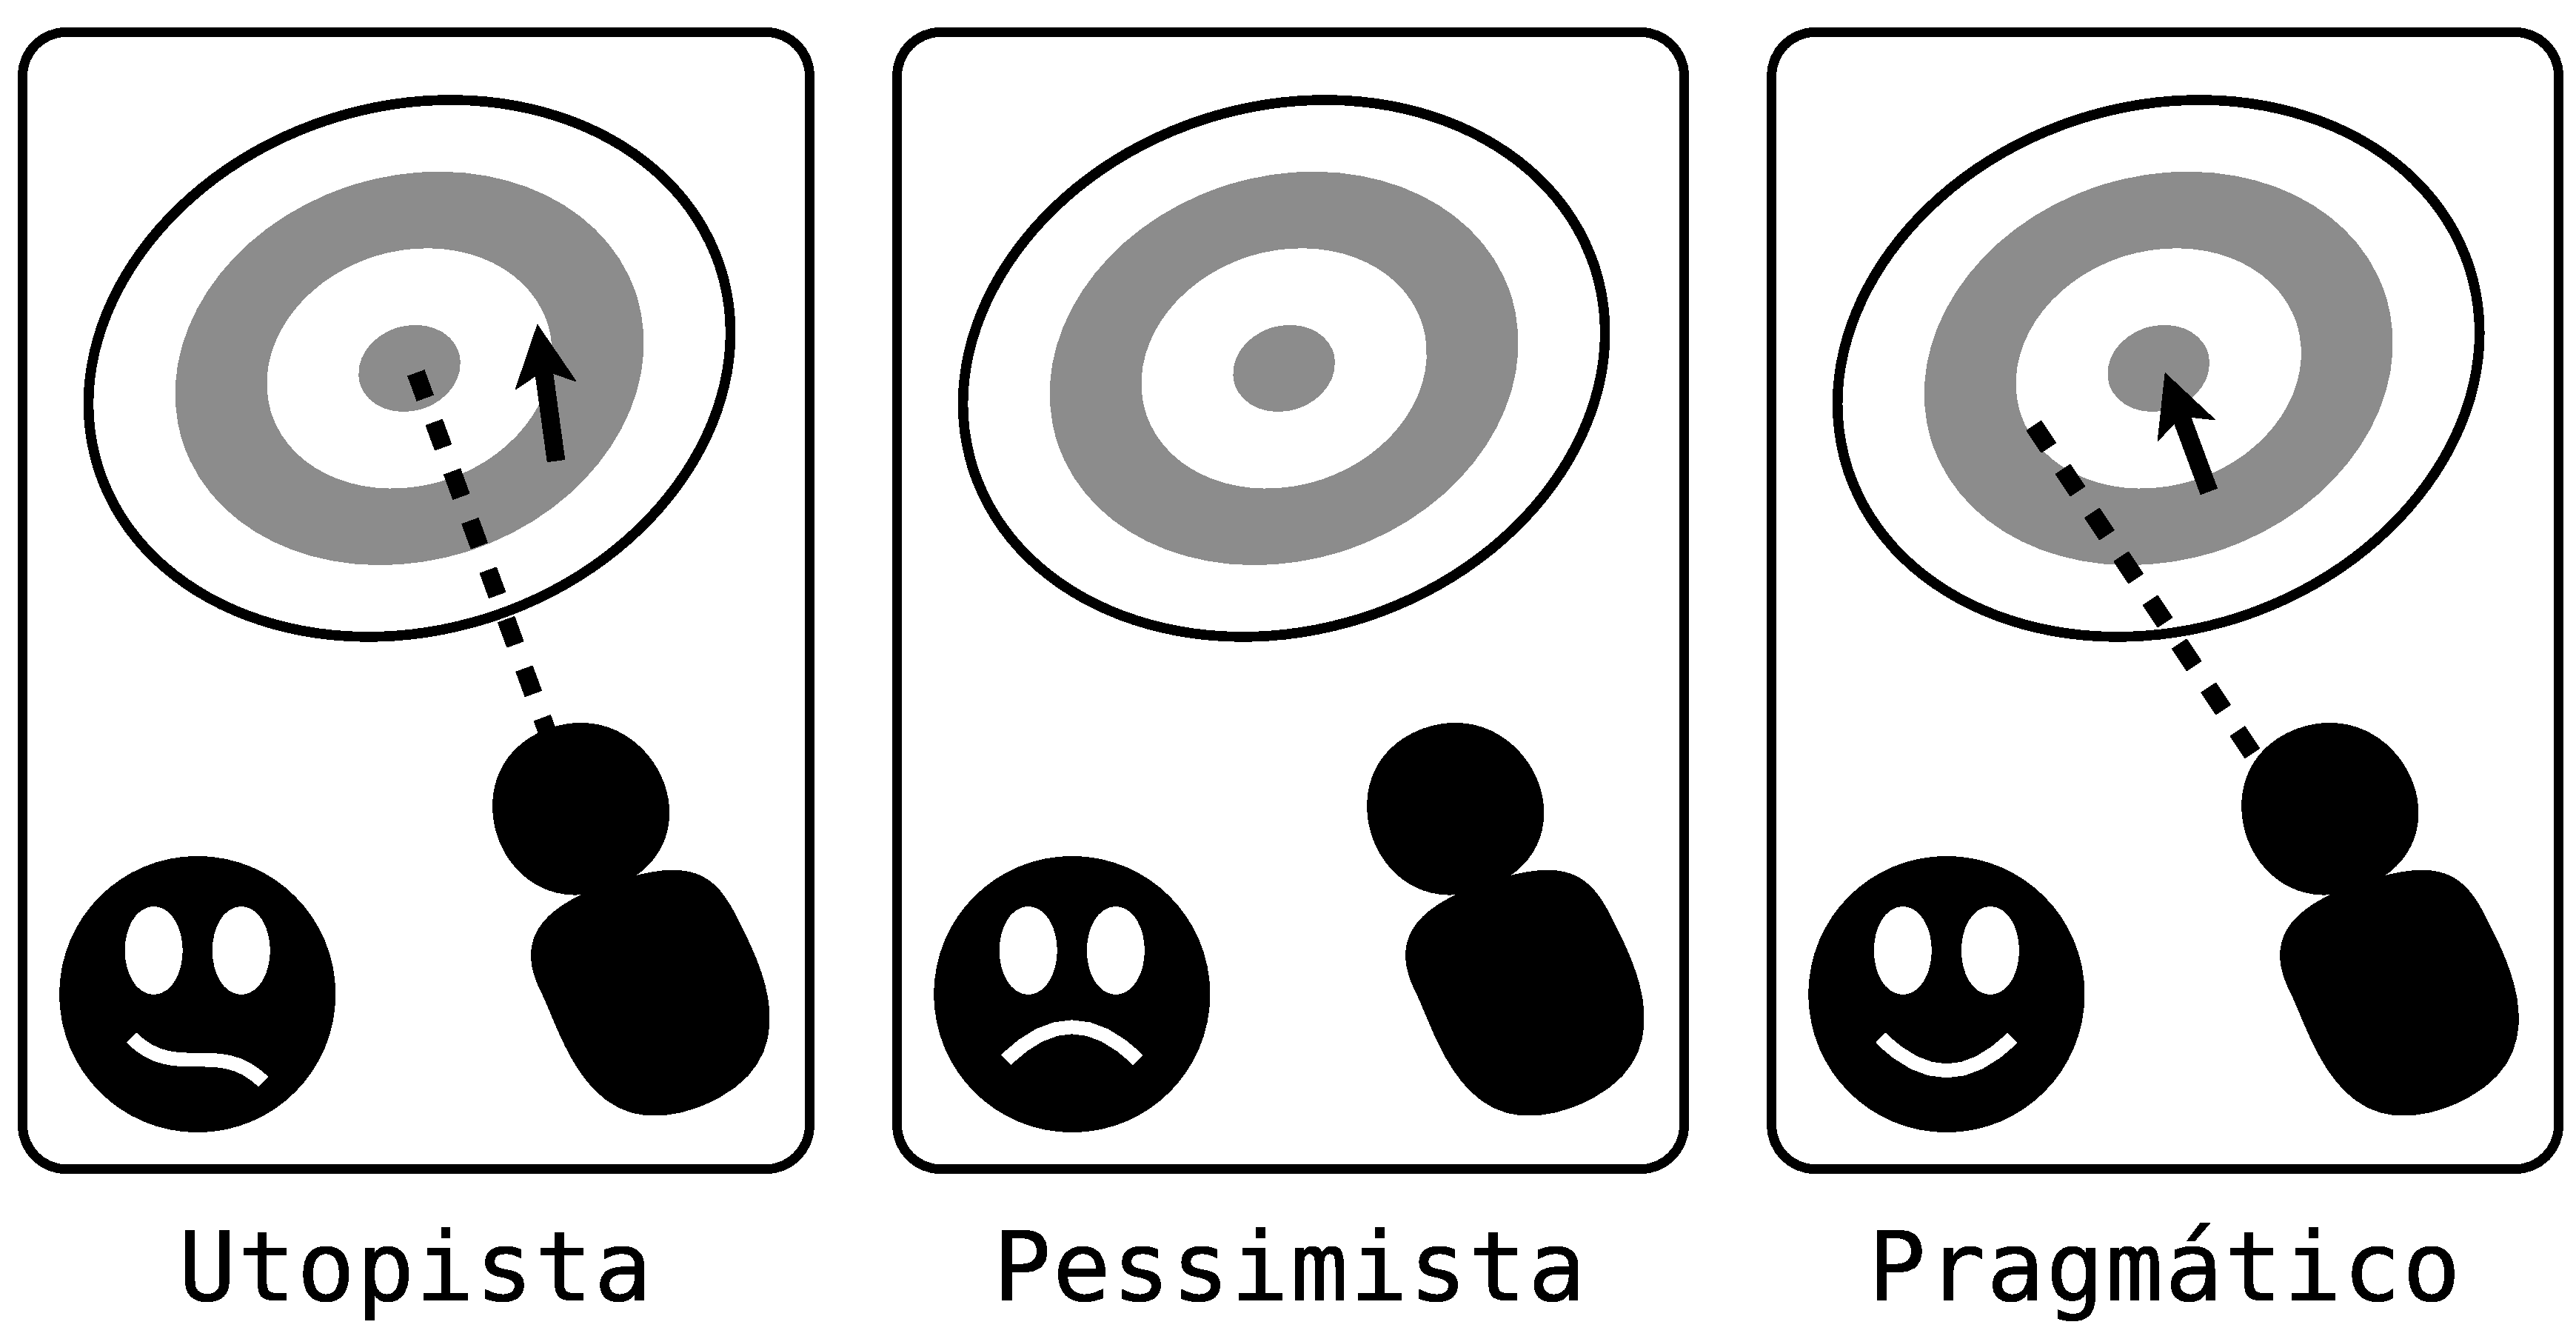
\includegraphics[width=0.7\textwidth]{chapters/cap-body-control/problema-generico-completo.eps}
\end{center}
\end{elaboracion}
\end{figure}

